\subsection{Nucleotide Binary Encoding} \label{background:nucleotide_binary_encoding}

DNA nucleotide sequences (described in section \ref{background:biology:dna_chromosomes_and_genomes}) inside computer software is commonly represented simply by a sequence of the 8 bit characters A, C, T and G (or alternatively the lowercase a, c, t and g).
This representation, however, is cumbersome to operate on and requires large amounts of memory to store.
To circumvent these issues, a widely adopted technique is to encode the nucleotides into binary form.
This leads to much quicker processing of nucleotide sequences and reduces the memory usage needed to store the sequences by 75\%.
This is achieved by realizing that only 2 bits, giving \textit{$2^2=4$} possible unique states, is enough to represent all of the four DNA nucleotides A, C, G and T.
The binary encoding can be extended further to represent whole nucleotide sequences in binary arrays.
For example, an integer array, if interpreted 2 consecutive bits at a time, can represent such a sequence.

\begin{figure}[ht!]
\begin{center}
\scalebox{1}{
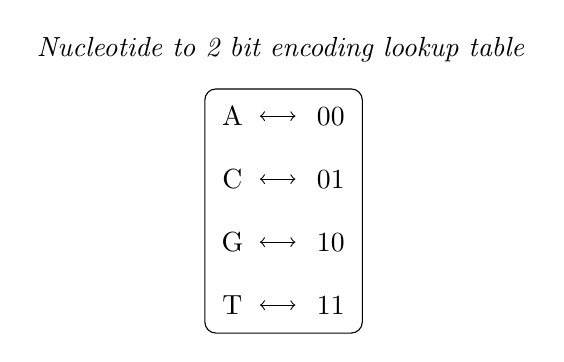
\begin{tikzpicture}
  \node at(.625,3.25)(title){\textit{Nucleotide to 2 bit encoding lookup table}};

  \node at(.65,1.195)[draw,rounded corners,minimum width=2cm,minimum height=3.1cm](lookuptable){};

  \node at(0,0)(){T};
  \node at(0,.8)(){G};
  \node at(0,1.6)(){C};
  \node at(0,2.4)(){A};

  \node at(1.25,0)(){11};
  \node at(1.25,.8)(){10};
  \node at(1.25,1.6)(){01};
  \node at(1.25,2.4)(){00};

  \draw [<->](.35,0) -- (.8,0);
  \draw [<->](.35,.8) -- (.8,.8);
  \draw [<->](.35,1.6) -- (.8,1.6);
  \draw [<->](.35,2.4) -- (.8,2.4);
\end{tikzpicture}
}

\scalebox{1}{
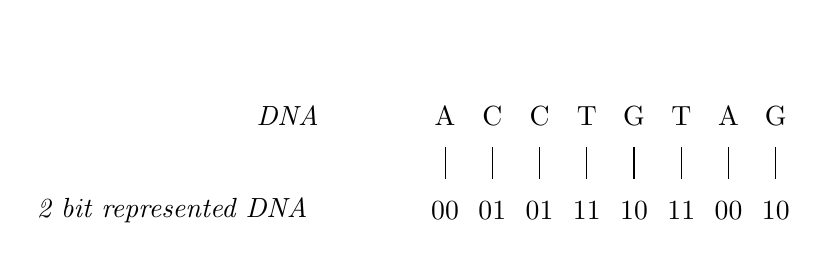
\begin{tikzpicture}
  \node at(0,1)(title){};

  \node at(-2,0)(){\textit{DNA}};
  \node at(-3.465,-1.2)(){\textit{2 bit represented DNA}};

  \node at(0,0)(){A};
  \node at(.6,0)(){C};
  \node at(1.2,0)(){C};
  \node at(1.8,0)(){T};
  \node at(2.4,0)(){G};
  \node at(3,0)(){T};
  \node at(3.6,0)(){A};
  \node at(4.2,0)(){G};

  \draw [](0,-.4) -- (0,-.8);
  \draw [](.6,-.4) -- (.6,-.8);
  \draw [](1.2,-.4) -- (1.2,-.8);
  \draw [](1.8,-.4) -- (1.8,-.8);
  \draw [](2.4,-.4) -- (2.4,-.8);
  \draw [](3,-.4) -- (3,-.8);
  \draw [](3.6,-.4) -- (3.6,-.8);
  \draw [](4.2,-.4) -- (4.2,-.8);

  \node at(0,-1.2)(){00};
  \node at(.6,-1.2)(){01};
  \node at(1.2,-1.2)(){01};
  \node at(1.8,-1.2)(){11};
  \node at(2.4,-1.2)(){10};
  \node at(3,-1.2)(){11};
  \node at(3.6,-1.2)(){00};
  \node at(4.2,-1.2)(){10};

\end{tikzpicture}
}
\caption{A lookup table showing how nucleotides can be encoded using 2 bits and a DNA nucleotide sequence represented both as plain characters as well as its 2 bit encoded representation. Recall that computers use 8 bits to represent a single nucleotide with a character, whilst the 2 bit encoding only needs 2 bits to represent a nucleotide.}
\label{background:nucleotide_binary_encoding:figures:nucleotide_binary_encoding}
\end{center}
\end{figure}
